The following figures show images of the preliminary CAD model for the legs. Note that some small features may be missing, and some were added on the pictures for clarity. There are also a few interfering parts that will need to be adjusted. Figure \ref{fig:leg_side} shows the leg in an extended position, which is taken as the worse case scenario for the torques applied on the legs.

\begin{figure}
    \centering
    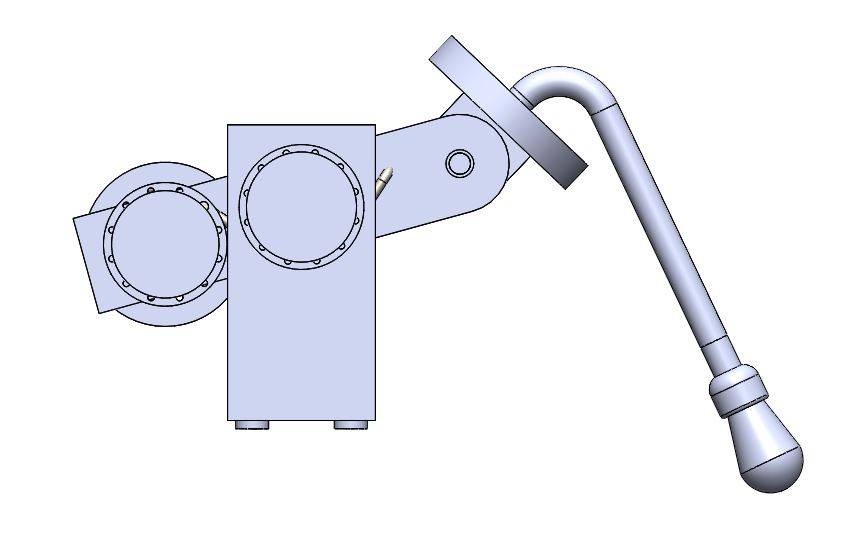
\includegraphics[width=0.8\textwidth]{2_DetailedDesign/img/LegSideView.JPG}
    \caption{Side view of leg assembly in extended position}
    \label{fig:leg_side}
\end{figure}

Figure \ref{fig:leg_side_sec} shows a side section view of the leg, with the bellow. Each leg now only has one bellow as the space between the two joints (knee and hip) is too small to accommodate two separate bellows. The side of the bellow with the largest diameter is going to be attached to the chassis. The smaller diameter side is attached to a circular part into which the tibia tube is press fit. 

\begin{figure}
    \centering
    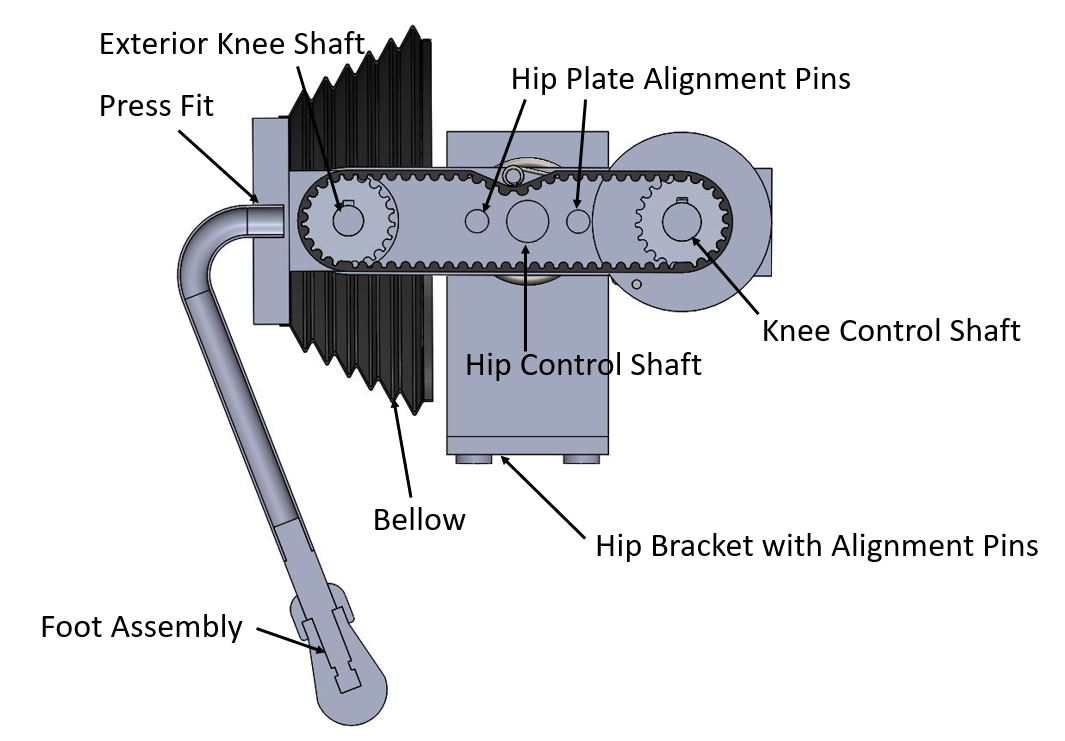
\includegraphics[width=0.8\textwidth]{2_DetailedDesign/img/LegSideSection_a.JPG}
    \caption{Side section of leg assembly with bellow}
    \label{fig:leg_side_sec}
\end{figure}

Figure \ref{fig:leg_top} gives a view of the assembly of the leg with the motors and harmonic drives. It also shows the torsion springs that were added to provide backdriving torque for when the robot is not moving. Note that the torsion springs on the hip control shaft should be holding on to the hip bracket as well as the hip plate. Their configuration will be changed to allow for that. Circular plates (spring supports) were added on each side of the pulley on the knee control shaft to allow for the attachment of the torsion springs.
Figure \ref{fig:leg_front} gives another view of the assembly.

\begin{figure}
    \centering
    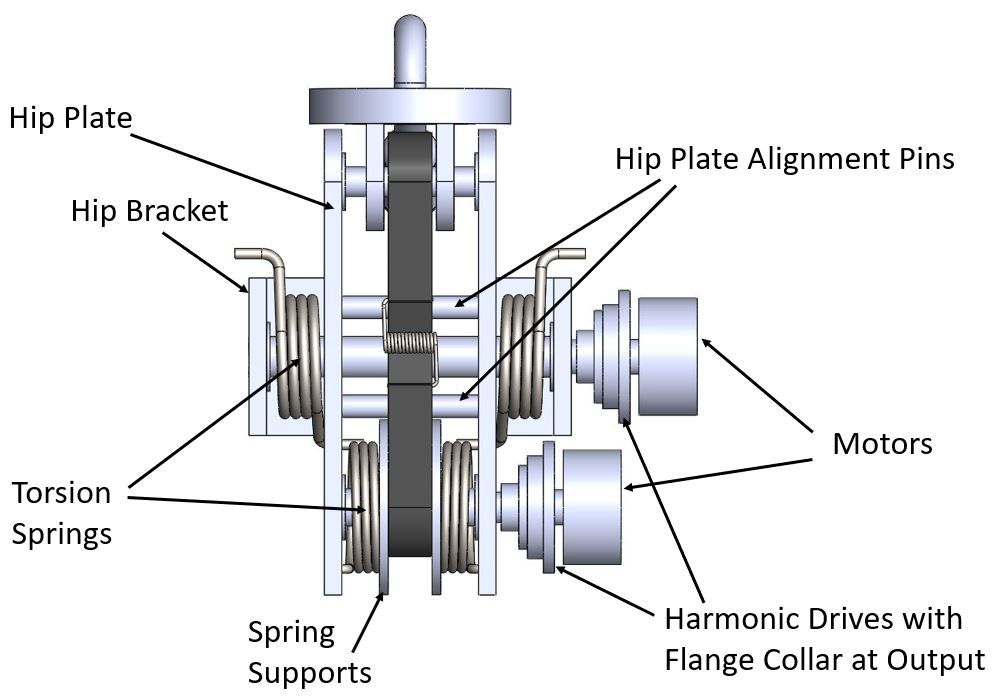
\includegraphics[width=0.8\textwidth]{2_DetailedDesign/img/LegTopView_a.JPG}
    \caption{Top view of leg assembly}
    \label{fig:leg_top}
\end{figure}

\begin{figure}
    \centering
    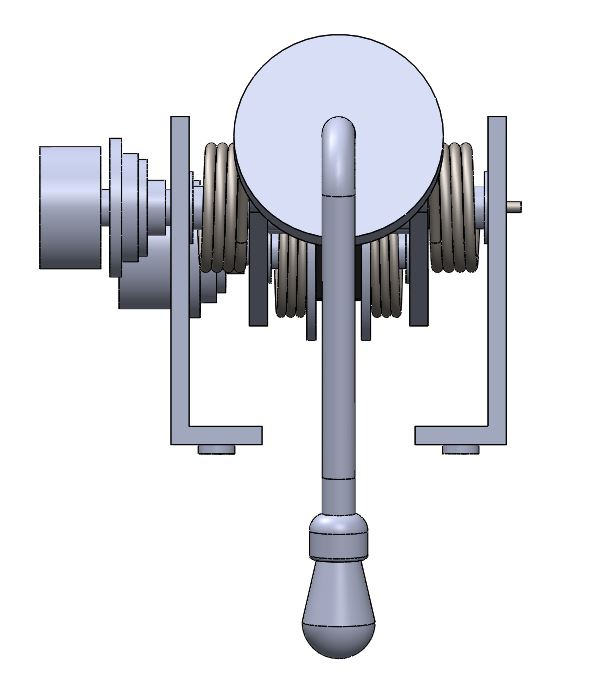
\includegraphics[width=0.5\textwidth]{2_DetailedDesign/img/LegFrontView.JPG}
    \caption{Front View of leg assembly}
    \label{fig:leg_front}
\end{figure}

As seen in the previous figures, the thigh member no longer consists of a tube. Instead, the machined hip and knee plates were joined and now consist of the thigh. Pins in between the two plates were added for alignment and sturdiness. A cross-section of a pin is shown in Figure \ref{fig:hip_alignment}.

\begin{figure}
    \centering
    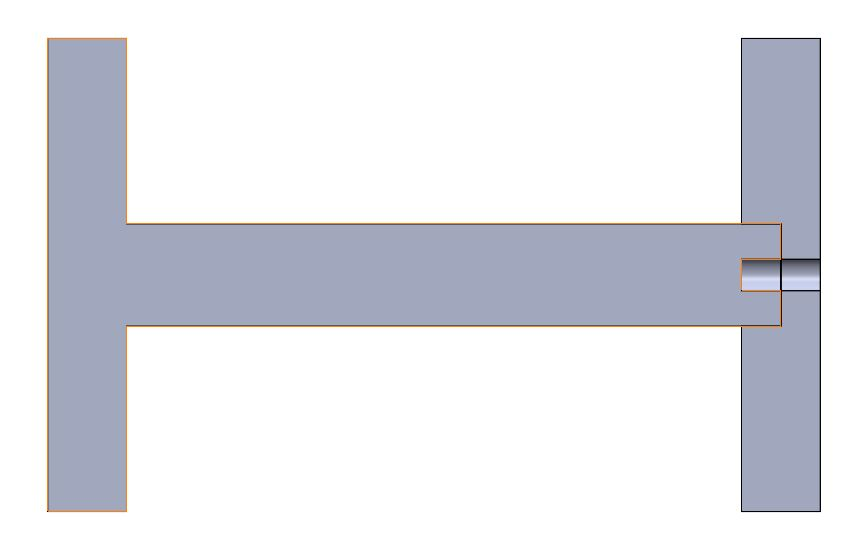
\includegraphics[width=0.5\textwidth]{2_DetailedDesign/img/HipPlateAlignment.JPG}
    \caption{Hip plate alignment pin section}
    \label{fig:hip_alignment}
\end{figure}

An updated version of the foot assembly is shown in Figure \ref{fig:foot}. The solid tube is going to be threaded to allow the compression cap to screw onto the silicone sock (the thread is drawn over the picture for now as it is not yet implemented in the CAD).

\begin{figure}
    \centering
    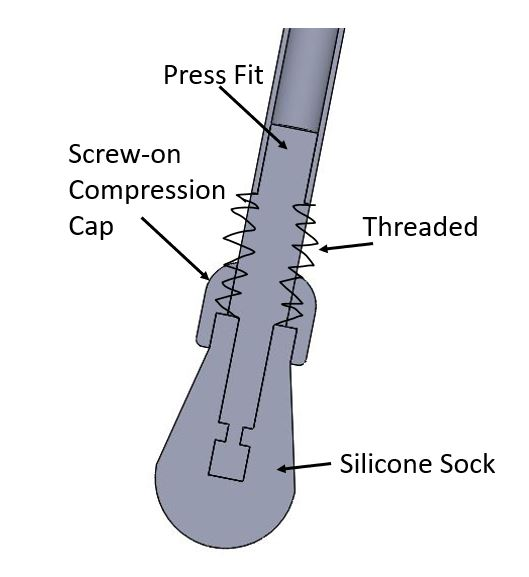
\includegraphics[width=0.6\textwidth]{2_DetailedDesign/img/Foot_a.JPG}
    \caption{Foot assembly}
    \label{fig:foot}
\end{figure}

Cross-sections of all three shafts along their axis are shown in Figures \ref{fig:shaft_knee}, \ref{fig:shaft_hipknee} and \ref{fig:shaft_hip}. Note that spacers and keys were added over the pictures as those features have not yet been implemented in CAD. Fasteners have not been included yet. For the knee shaft, there should be no clearance between the pulley and the tibia connection, and they are to be connected with fasteners. Note also that the torsion springs on the knee control shaft have some interference with neighbouring parts, which will be fixed.

\begin{figure}
    \centering
    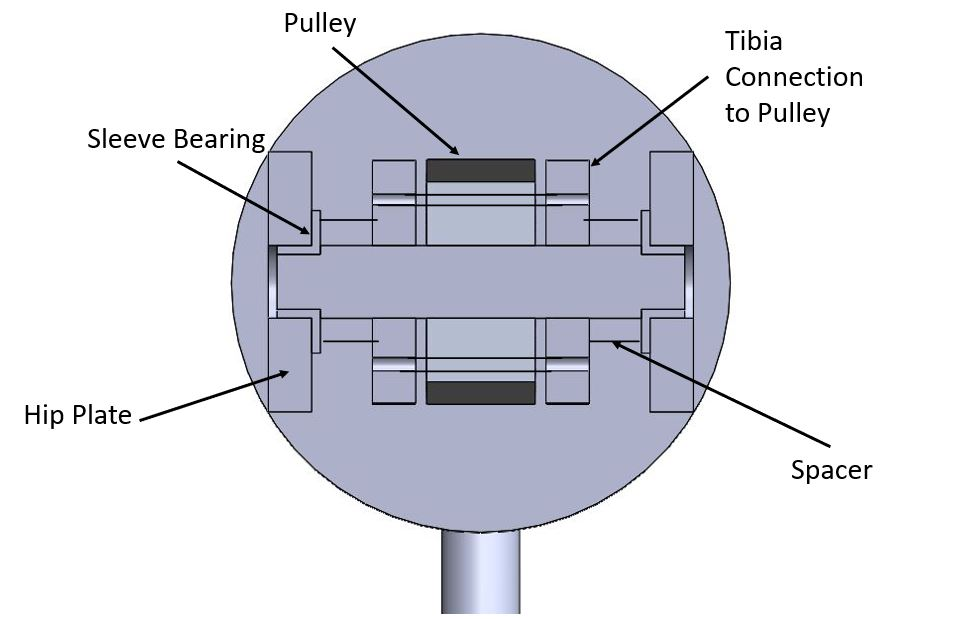
\includegraphics[width=0.8\textwidth]{2_DetailedDesign/img/KneeShaft_a.JPG}
    \caption{Exterior knee shaft section}
    \label{fig:shaft_knee}
\end{figure}

\begin{figure}
    \centering
    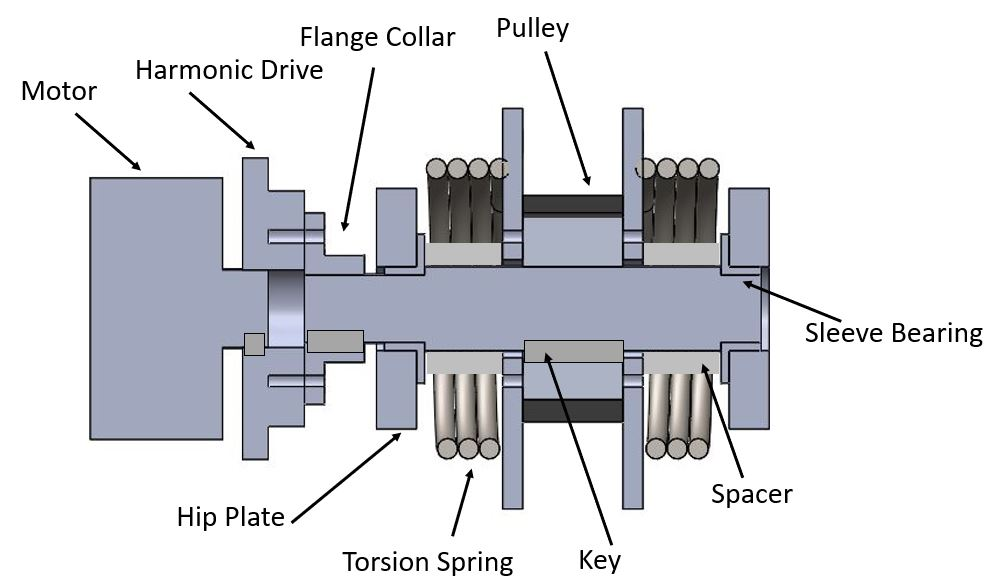
\includegraphics[width=\textwidth]{2_DetailedDesign/img/HipKneeShaft_a.JPG}
    \caption{Knee control shaft section}
    \label{fig:shaft_hipknee}
\end{figure}

\begin{figure}
    \centering
    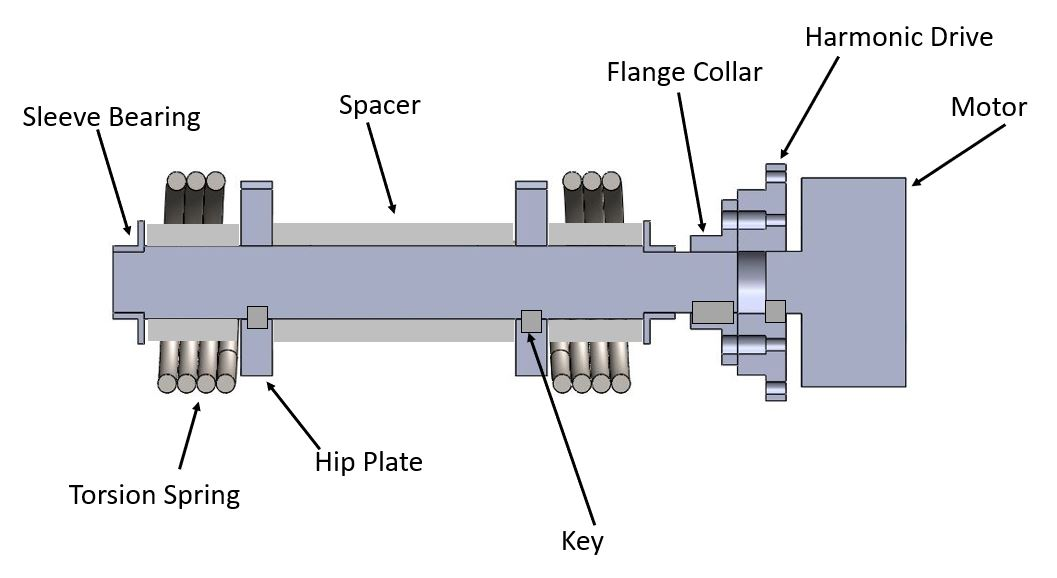
\includegraphics[width=\textwidth]{2_DetailedDesign/img/HipShaft_a.JPG}
    \caption{Hip control shaft section}
    \label{fig:shaft_hip}
\end{figure}

The timing belt's tensioner has been drawn in two possible configurations. The first scenario presented on Figure \ref{fig:beltSlack} is when the slack side of the belt is the top which occurs when the knee is holding the robots weight or when the tibia is moving downward. The other scenario illustrated on Figure \ref{fig:beltTight} represents what would happen if the belt were to overtighten and cancel the effects of the torsion spring.

\begin{figure}
    \centering
    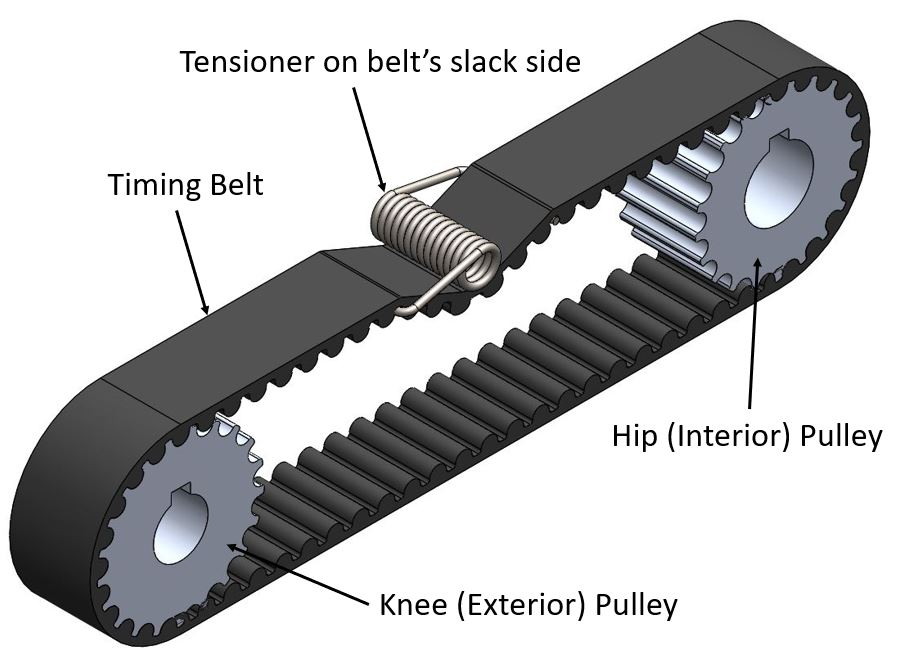
\includegraphics[width=0.7\textwidth]{2_DetailedDesign/img/BeltPulleySlack_a.JPG}
    \caption{Isometric view of belt and pulleys with a tensioner on the belt's slack side}
    \label{fig:beltSlack}
\end{figure}

\begin{figure}
    \centering
    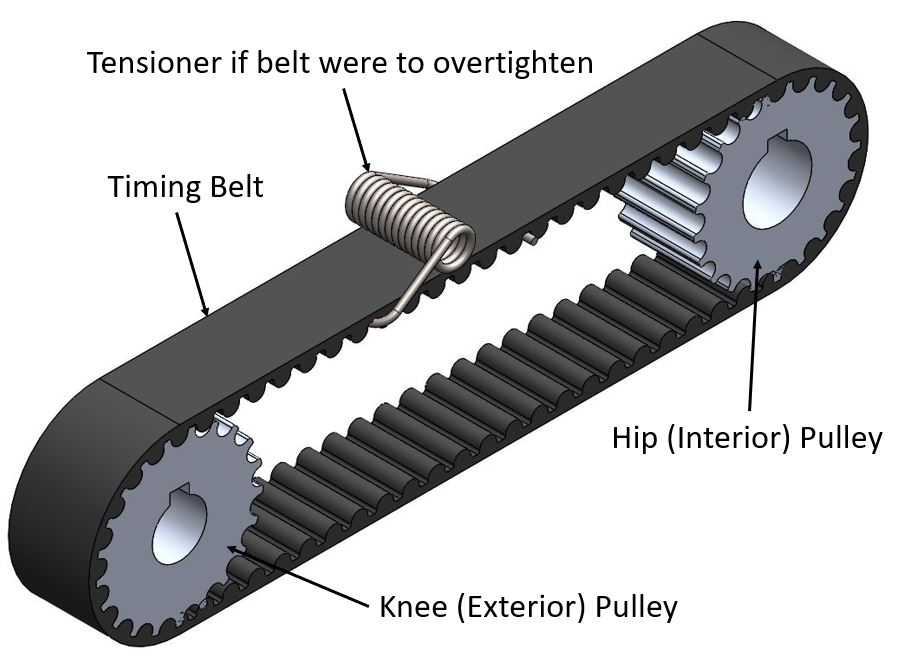
\includegraphics[width=0.7\textwidth]{2_DetailedDesign/img/BeltPulleyTight_a.JPG}
    \caption{Isometric view of belt and pulleys with a tensioner on the belt's tight side}
    \label{fig:beltTight}
\end{figure}
